\documentclass[a4paper,10pt]{article}
\usepackage{listings}
\usepackage{color}
\usepackage{graphicx}
\usepackage{textcomp}

\lstset{language=Java}
\lstset{breaklines=true, numbers=left}
\lstset{tabsize=4}

\definecolor{CommentColor}{rgb}{0,0.5,0} 
\definecolor{KeywordColor}{rgb}{0,0,0.5}

\lstset{commentstyle=\scriptsize\color{CommentColor}\itshape}
\lstset{keywordstyle=\scriptsize\color{KeywordColor}\bfseries}
\lstset{basicstyle=\scriptsize}
\lstset{identifierstyle=\scriptsize}
\lstset{stringstyle=\scriptsize}

% \lstset{basicstyle=\ttfamily}

\definecolor{lightblue}{rgb}{0.7,0.7,1}
\definecolor{lightyellow}{rgb}{1,1,0.5}
\definecolor{lightred}{rgb}{1,0.5,0.5}
\definecolor{lightgreen}{rgb}{0.7,1,0.7}

\newcommand{\src}[1]{\texttt{#1}}

% thanks to http://www.alfredklomp.com/programming/tex/macros/
\long\def\greybox#1#2#3{%
    \newbox\contentbox%
    \newbox\bkgdbox%
    \setbox\contentbox\hbox to \hsize{%
        \vtop{
            \kern\columnsep
            \hbox to \hsize{%
                \kern\columnsep%
                \advance\hsize by -2\columnsep%
                \parbox{0.1\hsize}{\includegraphics[width=\hsize]{#2}}%
                \hspace{0.025\hsize}%
                \advance\hsize by -0.125\hsize%
                \setlength{\textwidth}{\hsize}%
                \vbox{
                    \parskip=\baselineskip
                    \parindent=0bp
                    \parbox[c]{\hsize}{#3}
                }%
                \kern\columnsep%
            }%
            \kern\columnsep%
        }%
    }%
    \setbox\bkgdbox\vbox{
	\color{#1}
        \hrule width  \wd\contentbox %
               height \ht\contentbox %
               depth  \dp\contentbox
	\color{black}
    }%
    \wd\bkgdbox=0bp%
    \vbox{\hbox to \hsize{\box\bkgdbox\box\contentbox}}%
    \vskip\baselineskip%
}

\newcommand{\designbox}[1]{\greybox{lightgreen}{design}{#1}}
\newcommand{\classbox}[1]{\greybox{lightyellow}{class}{#1}}
\newcommand{\warningbox}[1]{\greybox{lightred}{stop}{#1}}
\newcommand{\infobox}[1]{\greybox{lightblue}{info}{#1}}

\title{DockingFrames 1.0.6 - Core}
\author{Benjamin Sigg}

\begin{document}

\maketitle
\tableofcontents
\newpage


\begin{abstract}
 \src{DockingFrames} is an open source Java Swing framework. This project allows to write applications with floating panels, meaning that the user can freely choose where to place the panels.

\src{DockingFrames} is divided into two projects, \src{Core} and \src{Common}. This document only covers \src{Core}, \src{Common} has its own guide.

The goal of this document is to provide any developer with a basic understanding of \src{DockingFrames}. One will not be able to rewrite the project after reading this document, but one will be able to start digging in the source.
\end{abstract}


\section{Notation}
This document uses various notations.

Any element that can be source code (e.g. a class name) and project names are written monospaced like this: \src{java.lang.String}. The package of classes and interfaces is rarely given since almost no name is used twice. The packages can be easily found with the help of the generated api documentation (JavaDoc).

\infobox{Tipps and tricks are listed in boxes.}

\warningbox{Important notes and warnings are listed in boxes like this one.}

\classbox{Implementation details, especially lists of class names, are written in boxes like this.}

\designbox{These boxes explain \textit{why} some thing was designed the way it is. This might either contain some bit of history or an explanation why some akward design is as bad as it first looks.}

\section{Basics}
The basic idea of \src{Core} is to have one object that controlls the framework, one object for each floating panel and one object for each area where a floating panel can be docked.

\classbox{The controller is a \src{DockController}, the floating panels are \src{Dockable}s and the dock-areas are \src{DockStation}s.}

\subsection{Hello World}
Let's start with a simple hello world. This application uses the three basic components, the example consists of valid code and can run:
\begin{lstlisting}
import javax.swing.JFrame;

import bibliothek.gui.DockController;
import bibliothek.gui.dock.DefaultDockable;
import bibliothek.gui.dock.SplitDockStation;
import bibliothek.gui.dock.station.split.SplitDockGrid;

public class HelloWorld {
	public static void main( String[] args ) {
		DockController controller = new DockController();

		SplitDockStation station = new SplitDockStation();
		controller.add( station );
	
		SplitDockGrid grid = new SplitDockGrid();
		grid.addDockable( 0, 0, 2, 1, new DefaultDockable( "N" ) );
		grid.addDockable( 0, 1, 1, 1, new DefaultDockable( "SW" ) );
		grid.addDockable( 1, 1, 1, 1, new DefaultDockable( "SE" ) );
		station.dropTree( grid.toTree() );
	
		JFrame frame = new JFrame();
		frame.add( station.getComponent() );
	
		frame.setDefaultCloseOperation( JFrame.EXIT_ON_CLOSE );
		frame.setBounds( 20, 20, 400, 400 );
		frame.setVisible( true );
	}
}
\end{lstlisting}
What happens here? In line \src{10} a \src{DockController} is created. The controller will handle things like drag and drop. All elements will be in his realm. In line \src{12} a new \src{DockStation} is created and in line \src{13} this station is registered as root station at the \src{DockController}.

Then in line \src{15-19} a few children for \src{station} are generated. To set the layout of those children a \src{SplitDockGrid} is used. \src{SplitDockGrid} takes a few \src{Dockable}s and their position and puts this information into a form that can be understood by \src{SplitDockStation} (line \src{19}). It would be possible to add the \src{Dockable}s directly to the station, but this is the easy way.

In line \src{21} a new frame is created and in line \src{22} our \src{DockStation} is added to the frame.

\infobox{More demonstration applications can be found in the big archive-file of \src{DockingFrames}. Each demonstration concentrates its attention on one feature of the framework.}

\subsection{Dockable}
A \src{Dockable} represents a floating panel, it consists at least of some \src{JComponent} (the panel it represents), some \src{Icon} and some text for a title. Each \src{Dockable} can be dragged by the user and dropped over a \src{DockStation}.

Clients can implement the interface \src{Dockable}, but it is much less painful just to use \src{DefaultDockable}. A \src{DefaultDockable} behaves in many ways like the well known \src{JFrame}: title, icon and panel can be set and replaced at any time.

A small example:
\begin{lstlisting}
DefaultDockable dockable = new DefaultDockable();
dockable.setTitleText( "I'm a JTree" );
Container content = dockable.getContentPane();
content.setLayout( new GridLayout( 1, 1 ) );
content.add( new JScrollPane( new JTree() ) );
\end{lstlisting}

\warningbox{If implementing \src{Dockable}, pay special attention to the api-doc. Some methods have a rather special behavior. It might be a good idea to subclass \src{AbstractDockable} or to copy as much as possible from it.}

\designbox{A careful analysis of \src{Dockable} reveals that there is no way for applications to store their own properties within a \src{Dockable} (unless using a subclass...). There are two reasons for this. First: if only using the default implementation, there is no need for clients to track these properties, store and load them or to delete them once they are no longer used. It is the responsibility of the framework to do so. Second: No special component within the framework or programming technique gets an unfair advantage over others, everything has to be designed in a way that it can work with any new, unknown, crazy other otherwise unexpected kind of \src{Dockable}.}

\subsection{DockStation}
\src{Dockable}s can never fly around for themself, they need a \src{DockStation} as anchor point. The relationship between \src{DockStation} and \src{Dockable} can best be described as parent-child-relationship. A \src{DockStation} can have many children, but a \src{Dockable} only one parent.

There are some classes which are \src{DockStation} and \src{Dockable} at the same time. They allow to build a tree of \src{DockStation}s and \src{Dockable}s. The number of such trees is \textit{not} limited to one.

There are different kind of \src{DockStation}s, each kind has its unique behavior and abilities.
\begin{description}
 \item[StackDockStation] The children are organized like on a \src{JTabbedPane}. Only one child is visible, but another can be made visible by clicking some button.
 \item[SplitDockStation] The children are organized like in a tree of \src{JSplitPane}s. All children are visible and the user can change the (relative) size of the \src{Dockable}s.
 \item[FlapDockStation] Much like \src{StackDockStation} but the one visible child pops up in its own window. This station can also show no \src{Dockable} at all.
 \item[ScreenDockStation] Shows each child in its own window.
\end{description}

Clients can implement new \src{DockStation}s. But be warned that the interface contains many methods and a lot of them require a lot of code. Don't expect to write less than 1000 lines of code.

A small example that builds a \src{StackDockStation}:
\begin{lstlisting}
StackDockStation stack = new StackDockStation();
stack.setTitleText( "Stack" );
stack.drop( new DefaultDockable( "One" ) );
stack.drop( new DefaultDockable( "Two" ) );
\end{lstlisting}
Some observations: \src{StackDockStation} is a \src{Dockable} as well, in line \src{2} the title is set. Two \src{DefaultDockable}s are put onto the station in lines \src{3,4}, the method \src{drop} is available in all \src{DockStation}s.

\warningbox{\src{DockStation}s are the most complex classes within the framework, they are also among the most important classes. It is very uncommon to subclass them or to write new ones. If you think you need to subclass a \src{DockStation}, be sure to have explored all other options.}

\subsection{DockController}
A \src{DockController} manages almost all the interactions between \src{Dockable}s and \src{DockStation}s. A \src{DockController} seldomly does a task by himself, but it always knows how to find an object that can do the task.

There can be more than one \src{DockController} in an application. Each controller has its own realm and there is no interaction between controllers. Most applications will need only one \src{DockController}.

Clients need to register the root of their \src{DockStation}-\src{Dockable}-trees. They can use the method \src{add} of \src{DockController} to do that. All children of the root will automatically be registered as well. If a \src{DockStation} is not registered anywhere, it just does not work properly. For \src{Dockable}s one could say that registration equals visibility. A registered \src{Dockable} can be seen by the user, an unregistered not.

\classbox{\src{DockController} uses other classes to handle tasks. Many of these classes can be observed by listeners. An incomplete list:

\src{DockRegister}: a list of all \src{Dockable}s and \src{DockStation}s.

\src{DockRelocator}: handles drag and drop operations, can create a \src{Remote} to play around without user interaction.

\src{DoubleClickController}: detects double clicks on \src{Dockable}s or on components which represent \src{Dockable}s.

\src{KeyBoardController}: detects \src{KeyEvent}s on \src{Dockable}s or on components which represent \src{Dockable}s.}

\warningbox{Never forget to register the root-\src{DockStation}(s) at the \src{DockController} using the method \src{add}.}

\designbox{Why not just one \src{DockController} implemented as singleton? A singleton would make many interfaces simpler, eliminating all the code where the controller is handed over to even the smallest object. On the other hand there is absolutely no reason to limit oneself to only one object and there are applications which need more than one controller. In the end not using a singleton just gives more flexibility.}

\subsection{DockFrontend}
\src{DockController} only implements the basic functionallity. While this allows developers to add new exciting shiny customized features, it certainly doesn't help those developers which just want to use the framework.

The class \src{DockFrontend} represents a layer before \src{DockController} and adds a set of helpful methods. Especially a ``close''-button and the ability to store and load the layout are a great help. \src{DockFrontend} replaces \src{DockController}, clients should add the root-\src{DockStation}s directly to the frontend, not to the controller. They can use the method \src{addRoot} to do so.

\warningbox{\src{DockFrontend} adds a few nice features but not enough to write an application without even bothering to have a look at \src{DockingFrames}. Developers which can live with not having absolute control over the framework should use \src{Common}. \src{Common} adds all those features which make a docking-framework complete, e.g. a ``minimize''-button}

\designbox{\src{DockFrontend} was written long after \src{DockController}. For the most part it just reuses code that already exists. It would be possible to write two applications with exact the same behavior once with and once without \src{DockFrontend}. The only thing that \src{DockFrontend} adds to the framework is a central hub where all the important features are accessible and a good set of default-values for various properties of the framework.}

\infobox{Use the methods called \src{setDefault...} to set default values for properties which will be used for \src{Dockable}s. I.e. whether \src{Dockable}s are hideable or not.}

\subsubsection{Close-Button}
In order to show the close-button clients need first to register their \src{Dockable}s. The method \src{addDockable} is used for that. Each \src{Dockable} needs a unique identifier that is used internally by \src{DockFrontend}. Later clients can call the method \src{setHideable} to show or to hide the close-button.

By calling the method \src{setShowHideAction} clients can make the buttons invisible for all \src{Dockable}s, note however that the \src{Dockable}s hideable-property is not affected by this method.

If clients want to control whether a \src{Dockable} can be closed, they should add a \src{VetoableDockFrontendListener} to the \src{DockFrontend}. This listener will be informed before a \src{Dockable} is made invisible and allows to cancel the operation.

\designbox{Why is the close-button not part of the very core of the framework? For one because the very core works on abstract levels and should not be made more complex with special cases like this button. There are also different implementations of this button and not all perform the same actions when pressed (this is especially true when using \src{Common}).}

\subsubsection{Storing the layout}
The methods \src{save}, \src{load}, \src{delete} and \src{getSettings} are an easy way to store and load the layout. This mechanism will be explained in detail in another chapter.

\section{Load and Save layouts}
The layout of an application means the position, size and relationships of all the \src{Dockable}s and \src{DockStation}s. To store this layout on a harddrive and later to load it again is a great help for the user, he does not need to setup the layout over and over again.

\src{DockingFrames} distinguishes between local and global layout information. Local information only describes the relationship between one \src{Dockable} and its parent, global information describes whole trees of elements. There are no algorithms which recreate a whole layout from a set containing local information, but there are also no algorithms which can place a \src{Dockable} in the tree using global information. So both kinds of data have their use.

\subsection{Local: DockableProperty}
Every \src{DockStation} can create a \src{DockableProperty}-object for one of its children. This \src{DockableProperty} contains the position and size of one child.

Some \src{DockStation}s are also \src{Dockable}s. Those stations are not only able to create \src{DockableProperties} for their children but their parents can create a property for them. These two properties can be strung together to form a chain describing the position of a grand-child on its grand-parent.

\subsubsection{Creation}
How to create a \src{DockableProperty}? One way is of course just to create new objects using \src{new XYProperty(...)}. The other way is to retreive them from some \src{DockStation}s and \src{Dockable}s:
\begin{lstlisting}
Dockable dockable = ...

DockStation root = DockUtilities.getRoot( dockable );
DockableProperty location = DockUtilities.getPropertyChain( root, dockable );
\end{lstlisting}
In line \src{1} we get some unknown \src{Dockable}. In line \src{3} the \src{DockStation} which is at the top of the tree of stations and \src{Dockable}s is searched. Then in line \src{4} the location of \src{dockable} in respect to \src{root} is determined.

\classbox{There are five \src{DockableProperties} present in the framework.
\begin{description}
 \item[StackDockProperty] for \src{StackDockStation}, contains just the index of the \src{Dockable} in the stack.
 \item[FlapDockProperty] for \src{FlapDockStation}, contains index, size and whether the \src{Dockable} should hold its position when not focused.
 \item[ScreenDockProperty] for \src{ScreenDockStation}, contains the boundaries of a \src{Dockable} on the screen.
 \item[SplitDockProperty] for \src{SplitDockStation}. This deprecated property contains the boundaries of a \src{Dockable} on the station.
 \item[SplitDockPathProperty] also for \src{SplitDockStation}. This new property contains the exact path leading to a \src{Dockable} in the tree that is used internally by the \src{SplitDockStation}.
\end{description}
}

\subsubsection{Usage}
How to apply a \src{DockableProperty}? Every \src{DockStation} has a method \src{drop} that takes a \src{Dockable} and its position. That might look like this:
\begin{lstlisting}
Dockable dockable = ...
DockStation root = ...
DockableProperty location = ...

if( !root.drop( dockable, location )){
  root.drop( dockable );
}
\end{lstlisting}
In lines \src{1-3} some elements that were stored earlier are described. In line \src{5} we try to drop \src{dockable} on \src{root}, if that fails we just drop it somewhere (line \src{6}).

\src{DockableProperty}s are not safe to use. If the tree of stations and \\\src{Dockable}s changes, then an earlier created \src{DockableProperty} might not be consistent anymore. The method \src{drop} of \src{DockStation} checks for consistency and returns \src{false} if a \src{DockableProperty} is no longer valid.

\warningbox{Always check the result of \src{drop}, if it is \src{false} then the operation was canceled by the station because the property is invalid.}

\subsubsection{Storage}
\src{DockableProperty}s can be stored either as byte-stream or in xml-format by a \src{PropertyTransformer}. A set of \src{DockablePropertyFactories} is used by the transformer to store and load properties. The factories for the default properties are always installed. If a developer adds new properties then he should use the method \src{addFactory} to install new factories for them.

\infobox{If using \src{DockFrontend} the method \src{registerFactory} can be used to add a new \src{DockablePropertyFactory}. This factory will then be used by global transformer of the frontent.}

\subsection{Global: DockSituation}
The layout of a whole set of \src{Dockable}s and \src{DockStation}s can be stored with the help of a \src{DockSituation}. A \src{DockSituation} is a set of algorithms that transform the layout information from one format into another, e.g. from the dock-tree (built by stations and \src{Dockable}s) to an xml-file. A \src{DockSituation} uses various factories to transform one format into another.

\subsubsection{Basic Algorithms}
Global layout information comes in four formats:
\begin{description}
 \item[dock-tree format] The set of \src{Dockable}s and \src{DockStation}s as they are seen by the user.
 \item[binary format] A file containing binary data. This file is normally written by a \src{DataOuputStream} and read by a \src{DataInputStream}.
 \item[xml format] A file containing xml. To write and read such a file the class \src{XIO} is used.
 \item[layout-composition format] An intermediate format that consists of a set of \src{DockLayoutComposition}s. These objects are organized in a tree that has the same form as the dock-tree.
\end{description}
To convert one format into another a \src{DockSituation} is used. If converting from \src{a} to \src{b} then a \src{DockSituation} will always first convert \src{a} to \src{layout-composition} and then \src{layout-composition} to \src{b}.

\warningbox{\src{DockSituation} always creates new files or new objects. In its basic form it is not able to reuse existing elements.}

A \src{DockSituation} uses different factories and strategies for these conversions:
\begin{description}
 \item[DockFactory] These factories are responsible to load or store the layout of a single \src{Dockable} or \src{DockStation}. Like \src{DockSituation} they need to support four formats. For one the dock-element they store or read, then binary- and xml-format and finally some object as intermediate formate. They are free to choose any kind of object as intermediate format.
 \item[AdjacentDockFactory] They function the same way as \src{DockFactories} but can be used for arbitrary dock-elements. \src{AdjacentDockFactories} are used to store additional information about elements, that can, but does not have to be, layout information.
 \item[MissingDockFactory] These are used when another factory is missing. The \src{MissingDockFactory} can try to read the xml-format or binary-format and convert it to the intermediate format.
 \item[DockSituationIgnore] This strategy allows a \src{DockSituation} to ignore dock-elements when storing the layout. That can be helpful if e.g. an application has \src{Dockable}s which show only temporary information that will be lost on shutdown anyway.
 \end{description}

A \src{DockSituation} can handle missing factories when reading xml or binary format. It first tries to use a \src{MissingDockFatory} to read the data, if that fails it either throws away the data (for \src{AdjacentDockFactories}) or stores the data in the layout-composition as ``bubble'' in its raw format. These ``bubbles'' can be converted later when the missing factories are found.

\classbox{A \src{DockLayoutComposition} contains a lot of information. First of all a list of children to build the tree. Then a list of \src{DockLayout}s which represent the information from \src{AdjacentDockFactories}. Each \src{DockLayout} contains a unique identifier for the factory and the data generated by the factory. Finally a \src{DockLayoutComposition} contains a \src{DockLayoutInfo} which represents the data of or for a \src{DockFactory}. A \src{DockLayoutInfo} either contains a \src{DockLayout} (the normal case) or some data in xml or binary format. The later case happens if a factory was missing while reading a file, the information gets stored until it can be read later.}

\infobox{The method \src{fillMissing} can be used to read ``bubbles'' in raw format. The method \src{estimateLocations} can be used to build \src{DockableProperties} for the elements. These are the positions were the elements would come to rest if the layout information were converted into a dock-tree.}

\subsubsection{Basic Usage}
How is a \src{DockSituation} utilized in order to load or store the layout of an application?

Each \src{Dockable} and each \src{DockStation} have a method \src{getFactoryID}. This method returns an identifier that has to match the unique identifier that is returned by the method \src{getID} of \src{DockFactory}. So the first step in using a \src{DockSituation} will always be to make sure that for any identifier a matching \src{DockFactory} is available. Clients will call the method \src{add} of \src{DockSituation} to do so.

\infobox{Default factories are installed for \src{DefaultDockable}, \src{SplitDockStation}, \src{StackDockStation} and \src{FlapDockStation}.}

\warningbox{The \src{ScreenDockStationFactory} for \src{ScreenDockStation} is not installed per default. This factory requires a \src{WindowProvider} to create the station, and since this provider cannot be guessed by \src{DockSituation} the factory is missing. Clients have to add \src{ScreenDockStationFactory} manually.}

Afterwards clients just have to call \src{write} or \src{writeXML} to write a set of \src{DockStation}s and their children. Clients can later call \src{read} or \src{readXML} to read the same map of elements. Note that every call to \src{read} or \src{readXML} will create a new set of \src{Dockable}- and \src{DockStation}-objects.

Let't give an example how to write an xml file:
\begin{lstlisting}
try{
	JFrame frame = ...
	DockStation root = ...

	DockSituation situation = new DockSituation();
	situation.add( new ScreenDockStationFactory( frame ) );
	situation.add( new MySpecialFactory() );

	Map<String, DockStation> map = new HashMap<String, DockStation>();
	map.put( "root", root );

	XElement xlayout = new XElement( "layout" );
	situation.writeXML( map, xlayout );

	FileOutputStream out = new FileOutputStream( "layout.xml" );
	XIO.writeUTF( xlayout, out );
	out.close();
}
catch( IOException ex ){
	ex.printStackTrace();
}
\end{lstlisting}
On line \src{2} the main-frame of the application is given and on line \src{3} the applications root \src{DockStation}. The first step is to create a new \src{DockSituation} on line \src{5} and add the missing \src{ScreenDockStationFactory} on line \src{6}. Then other factories that are not part of \src{DockingFrames} but the application itself can be added like on line \src{7}. On lines \src{9, 10} a map with all the root-stations of the application is built up. Then on line \src{12} we prepare for writing in xml-format by creating a \src{XElement}. The situation converts the dock-tree to xml-format in line \src{13}. Finally on lines \src{15-17} the xml-tree is written into a file ``layout.xml''.

The next example shows how reading from binary format can look like:
\begin{lstlisting}
try{
	JFrame frame = ...

	DockSituation situation = new DockSituation();
	situation.add( new ScreenDockStationFactory( frame ) );
	situation.add( new MySpecialFactory() );

	FileInputStream fileStream = new FileInputStream( "layout" );
	DataInputStream in = new DataInputStream( fileStream );

	Map<String, DockStation> map = situation.read( in );

	in.close();

	SplitDockStation station = (SplitDockStation)map.get( "root" );
	frame.add( station.getComponent() );
}
catch( IOException ex ){
	ex.printStackTrace();
}
\end{lstlisting}
What happens here? In line \src{2} the main frame of the application is defined. In lines \src{4-6} a \src{DockSituation} is set up. In lines \src{8, 9} a file is opened. In line \src{11} that file gets read by the \src{DockSituation} and a map that was earlier given to \src{write} is returned. In line \src{15} the fact that \src{map} was earlier given to \src{write} is used to guess that there is a \src{SplitDockStation} with key ``root'' in the map. Finally in line \src{16} that station is put onto the main-frame which now shows the new elements.

\subsubsection{Extended Algorithms}
The major drawback of the basic algorithms is that they always create new \src{Dockable}s and \src{DockStation}s. As a result it is nearly impossible to just change the layout while an application is running, a layout can only be loaded on startup. \src{PredefinedDockSituation} builds upon \src{DockSituation} and extends the algorithms in a way that the can reuse existing dock-elements.

The extended version uses a special \src{DockFactory}, called \src{PreloadFactory}, that is wrapped around the factories providied by the client. Writing does not change much, the \src{PreloadFactory} delegates the work just to the original \src{DockFactory}. Reading is more interesting. The \src{PreloadFactory} forwards the dock-element to reuse to the the original \src{DockFactory} which then updates the layout of the element.

A side effect of this implementation is, that for the basic \src{DockSituation} no factories seem ever to be missing. In fact the issue of missing factories is just moved to the \src{PreloadFactory}. The \src{PreloadFactory} can however store data in its raw format if necessary.

\classbox{A \src{PreloadFactory} uses a \src{PreloadedLayout} as intermediate format. This \src{PreloadedLayout} contains the unique identifier of the original \src{DockFactory} and a \src{DockLayoutInfo}. The \src{DockLayoutInfo} contains either data in raw format or in the intermediate format of the original factory.}

What happens if a \src{PredefinedDockSituation} finds layout information for an element, has all the necessary factories but not the element itself? The default behavior is to ignore the information. However it is possible to use backup-\src{DockFactories}. These backup factories will create new elements if they were missing. They are also used when reading raw format and the original factory is missing. These backup factories are added through \src{addBackup}, they have to use a \src{BackupFactoryData} as intermediate format.

\warningbox{Note that the \src{MissingDockFactory} of \src{DockSituation} is not used for elements that were predefined on writing, because for those elements the \src{PreloadFactory} - which is never missing - was used.}

\designbox{The existence of these two sets of algorithms, basic and extended, lays in the history of \src{DockingFrames}. First the basic algorithms were written. They did their job well for small applications. But when applications began to grow it became evident that their were not sufficient. Instead of rewriting them another layer was added. The division in two sets of algorithms has also the advantage of reduced complexity.

The recovery mechanisms for missing factories were introduced for version 1.0.7. They are not yet satisfying and it is likely that they will be changed again in future versions.}

\subsubsection{Extended Usage}
\src{PredefinedDockSituation} is used in the same way as \src{DockSituation}. The only difference is the possibility to predefine elements. The method \src{put} can be used for that. This method expects a unique identifier for any new element.

An example can look like this:
\begin{lstlisting}
	DockStation rootStation = ...
	Dockable fileTreeDockable = ...
	Dockable contentDockable = ...

	PredefinedDockSituation situation = new PredefinedDockSituation();

	// setup situation {...}

	situation.put( "root", rootStation );
	situation.put( "file-tree", fileTreeDockable );
	situation.put( "content", contentDockable );

	// read or write {...}
\end{lstlisting}
In lines \src{1-3} some \src{DockStation}s and \src{Dockable}s are defined. These are the elements that are always present and need not to be recreated when loading a layout. In line \src{5} a new \src{PredefinedDockSituation} is created. Then the basic setup (adding factories, ...) is done in line \src{7}. In the lines \src{9-11} the predefenied elements are added to the situation. For each of them a unique identifier is choosen. Finally in line \src{13} we can either write or read the layout.

\infobox{Any \src{String} can be used as unique identifier. Small identifiers with no special characters are however much less likely to attract any kind of trouble.}

\subsection{DockFrontend}
\src{DockFrontend} offers storage for local and for global layout information. Clients need to register their \src{Dockable}s through \src{addDockable} if they want access to the full range of storage-features.

\subsubsection{Local}
Whenever \src{hide} is called for a registered \src{Dockable} its local position gets stored. If later \src{show} is called this position is reapplied and the element shows up at the same (or nearly the same) location it was earlier. This local information can also be stored in xml- or binary-format. The methods \src{write}, \src{writeXML}, \src{read} and \src{readXML} will take care of this.

\subsubsection{Global}
\src{DockFrontend} internally uses a \src{PredefinedDockSituation} to store the global layout. All root-\src{DockStation}s and all registered \src{Dockable}s are automatically added to this situation. The global layout can either be stored on disk using the methods \src{write}, \src{writeXML}, \src{read} and \src{readXML} or it can be stored in memory. It is possible to store more than just one layout in memory and allow the user to choose from different layouts. There are methods to interact with the layouts in memory:

\begin{description}
 \item[save] Saves the current layout in memory. Clients can provide a name for the layout or use the name of the last loaded layout.
 \item[load] Loads a layout. The name of the layout is used as key.
 \item[delete] Deletes a layout from memory.
 \item[getSettings] Gets a set of names for the different layouts.
 \item[getCurrentSetting] Gets the name of the layout that is currently loaded, can be \src{null}.
 \item[setCurrentSetting] If there is a layout with the name given to this method than that layout is loaded. Otherwise the current layout gets saved with the new name.
\end{description}

The layouts that are in memory can be stored persistent as well.

\subsubsection{Missing Dockables}
The default behavior of \src{DockFrontend} is to through away information for missing \src{Dockable}s. It is however possible to change that behavior.

If data needs to be stored for a missing \src{Dockable} then \src{DockFrontend} uses an ``empty entry''. Clients can define new empty entries by invoking the method \src{addEmpty}. Existing entries can be removed with \src{removeEmpty}, with \src{listEmpty} all empty entries can be accessed. Once an entry has been marked as ``empty'' it can switch between filled and empty as many times as necessary without loosing its layout information. The \src{DockFrontend} can even store data in raw xml or binary format and convert this data later once an appropriate \src{DockFactory} becomes known.

\infobox{``Empty entries'' are best to be used if a client already knows the identifiers of all the \src{Dockable}s that can eventually be registered at the \src{DockFrontend}.}

Another way is to register backup-\src{DockFactories} by calling the method \src{registerBackupFactory}. These factories will create new \src{Dockable}s which are then automatically registered.

\infobox{A backup-factory is the strongest weapon against missing information. If there is a possibility to use them, use them.}

And finally there is the \src{MissingDockableStrategy} which can be set using \src{setMissingDockableStrategy}. This strategy enables or disables to automatic processes.
\begin{itemize}
 \item It allows to create ``empty entries'' automatically. There are two methods \src{shouldStoreShown} and \src{shouldStoreHidden} which have to check the identifiers and to return \src{true} to allow a new empty entry.
 \item It allows to use new \src{DockFactories} as soon as they become known. Normally \src{DockFrontend} does not change the layout without the explizit command from a client (by invoking \src{setSetting} directly or indirectly). If \src{shouldCreate} returns \src{true} however \src{DockFrontend} will update the layout as soon as enough information is available to do so.
\end{itemize}

\infobox{\src{MissingDockableStrategy} should be used when no information about what is missing is available. It allows to run a ``do whatever is possible''-strategy.}

\warningbox{If a strategy allows to store anything and a client often uses different identifiers for their \src{Dockable}s, then layouts will start to grow and never stop. Don't forget to delete outdated information.}

\classbox{The interface \src{MissingDockableStragey} offers two default implementations: \src{DISCARD\_ALL} and \src{STORE\_ALL}. The first implementation is set as default and allows nothing, the second one allows everything.}

\section{Actions} \label{sec:actions}
All \src{Dockable}s can be associated with some actions. An action normally appears as some kind of button in the title of a \src{Dockable}, they can however appear at other places as well. There are different types of actions, some may behave like a \src{JButton} others like a \src{JCheckBox}, clients can add new types.

\begin{figure}[h]
\centering
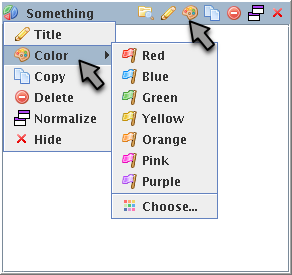
\includegraphics[scale=0.5]{actions}
\caption{A \src{Dockable} with a few \src{DockAction}s in its title and on a popup menu. The action marked by an arrow is the same object just shown in different views.}
\label{fig:actions}
\end{figure}

Actions are represented by the interface \src{DockAction}. Each \src{Dockable} has a list of them represented by a \src{DockActionSource}.

If some component wants to show some actions it firsts asks a \src{Dockable} for its global \src{DockActionSource}. It then asks each \src{DockAction} of that list to create a view that fits to the component. A title will ask for another kind of view than a menu. At any time actions can be added or removed from the \src{DockActionSource} and any component showing actions will react on these events.

\classbox{The interface \src{DockAction} is quite simple. Two methods to install (\src{bind}) and to uninstall (\src{unbind}) the action. One method to create new views (\src{createView}) and one method to trigger an action programatically (\src{trigger}). More useful are the many subclasses and subinterfaces. \src{StandardDockAction} introduces icons, text and tooltip. Five subinterfaces for \src{StandardDockAction} exist and for all of them a default-view is provided.}

\designbox{There are three levels in the design of \src{DockAction} and its subclasses. First there is \src{DockAction} which allows almost any kind of \src{Component} to be used as view. Second there are subinterfaces for the standard tasks, the framework provides views for them. Third are real implementations of the second-level interfaces. Some interfaces are implemented in more than one action for different styles of aplication organization.}

\subsection{Show Actions}
Assuming one has a \src{DockAction} (more about different kind of actions is in the next chapter) how can the framework be advised to show it? 

\subsubsection{List of Actions}
\src{DockAction}s never travel alone in this framework. They always travel with other actions in a \src{DockActionSource}. Actions can be added or removed from \src{DockActionSource}s at any time and modules showing actions will react on this.

Most methods of \src{DockActionSource} can be understood without explanation. The method \src{getLocationHint} is an exception. It returns a  \src{LocationHint} which is used to order several \src{DockActionSources} into a list (and treat them as one big \src{DockActionSource}). Clients which implement an \src{ActionOffer} can also introduce new kind of \src{LocationHint}s.

\classbox{\src{LocationHint}s consists of an \src{Origin} and a \src{Hint}. The hint tells the preferred location in respect to other elements, the origin are used if multiple hints collide. New \src{Hint}s and \src{Origin}s can be written.}

\subsubsection{Source of Actions}
Actions haf different sources, each kind of source has a specific purpose.

\begin{itemize}
 \item The \textbf{local action source} is part of every \src{Dockable}. This source is accessed through \src{getLocalActionOffers}. If \src{AbstractDockable} or a subclass like \src{DefaultDockable} is used then \src{setLocalActionOffers} allows to quickly set and exchange the actions. This source of actions should be used for actions that are closely linked with some \src{Dockable}.
 \item \src{ActionGuard}s can add actions to every \src{Dockable}. An \src{ActionGuard} is added to a \src{DockController} through \src{addActionGuard}. Its method \src{react} will be called whenever the actions of a \src{Dockable} are searched. If \src{react} returns \src{true} them the method \src{getSource} is called which adds the actions. This source of actions is intended either for general purpose action or for actions which need a special position in the list of actions (like a close-action needs to be at the very right end).
 \item Every \src{DockStation} can add \textbf{direct} and \textbf{indirect action offers} to its children. For this \src{DockStation} has two methods \src{getDirectActionOffers} and \src{getIndirectActionOffers}. \textbf{Direct action offers} are used only for true children, \src{indirect action offers} can be applied to grand-children as well. These sources of actions is intended for actions that are linked to a \src{DockStation}, like the maixmimze-action that can be seen on a \src{SplitDockStation}.
\end{itemize}

Two mechanisms are responsible for collecting all the actions form these different sources and o put them into one list. Clients can adjust these mechanisms even to a point where they no longer collect actions but introduce their own actions.

\begin{itemize}
 \item Every \src{DockController} has at least one \src{ActionOffer}. An \src{ActionOffer} has two methods, \src{interested} tells whether the offer is interested in managing a certain \src{Dockable} and \src{getSource} collects the actions of an interesting \src{Dockable}. The primary function of an \src{ActionOffer} is to order the various sources. It is up to the offer to decide how to actually do the sorting. The default \src{ActionOffer} uses the \src{LocationHint} which is attached to every \src{DockActionSource}.

Clients can use \src{addActionOffer} and \src{setDefaultActionOffer} to change the offers of a \src{DockController}. The public method \src{listOffers} then advises the controller to use its offers, clients however should not call this method directly. They should call \src{getGlobalActionOffers} of \src{Dockable}.

 \item Modules which need a list of actions call \src{getGlobalActionOffers} from \src{Dockable}. This method is the ultimate piece of code which decides what to show. If need by this method can ignore anything else that has been said in this chapter and introduce its very own mechanism to collect actinos. Most \src{Dockable}s however will create a field holding a \src{HierarchyDockActionSource}. This special source observes the hierarchy of a \src{Dockable} and changes its content automatically. \src{Dockable}s using \src{HierarchyDockActionSource} should \src{bind} the source. They need to call \src{update} if their own local action source is exchanged. 
\end{itemize}

\warningbox{It is generally a bad idea to write \src{DockActionOffer}s or \src{getGlobalActionOffer} methods which do not just collect actions. There are already mechanisms to introduce \src{DockAction}s and they should suffice for every possible situation.}

\subsection{Standard Actions}
There are a number of standard actions in the framework. Clients can either subclass them or instantiate and add listeners to them. A user would put the actions into six groups:
\begin{description}
 \item[Button] If the user clicks this action then always the same happens. The interface \src{ButtonDockAction} collects all the buttonlike actions.
 \item[Checkbox] When triggered it changes some property from \src{true} to \src{false} or from \src{false} to \src{true}. All actions with this behavior implement the interface \src{SelectableDockAction}.
 \item[Radiobutton] Like a group of checkboxes, but only one radiobutton can be selected within that group. Like checkboxes all these actions are represented by \src{SelectableDockAction}. Several radiobuttons can be linked together with the help of a \src{SelectableDockActionGroup}.
 \item[Menu] A menu just contains a list of other \src{DockAction}s. These other actions are normally hidden and only shown if the user wants to see them. Menus are implementing the interface \src{MenuDockAction}.
 \item[Drop-down-button] Like a menu but the last triggered action can be triggered again without opening the menu. The interface \src{DropDownAction} represents these special menus.
 \item[Separator] A separator just is a line, a graphical element to divide a set of actions into subsets. Separators are implemented through the class \src{SeparatorAction}.
\end{description}

\subsubsection{Simple actions}
Simple actions are a set of classes that implement the various action-interfaces. These simple actions do not have any advanced features and should be quite simple to use. An example might be the following code:

\begin{lstlisting}
public class ExampleAction extends SimpleButtonAction{
	public ExampleAction() {
		setText( "Run..." );
		setIcon( new ImageIcon( "example.png" ) );
		setTooltip( "Run the example" );
	}

	@Override
	public void action( Dockable dockable ) {
		System.out.println( "kabum" );
	}
}
\end{lstlisting}

Here the class \src{SimpleButtonAction} is used. The action is subclassed by \src{ExampleAction}. In lines \src{3-5} properties like the icon are set. The subclass overrides the method \src{action} (lines \src{9-11}) which is invoked every time when the user presses the button.

The available simple actions are:
\begin{itemize}
	\item \src{SimpleButtonAction}: For creating buttons. Can either be subclassed (like in the example above) or just instanciated. Clients can add instances of the well known \src{ActionListener}s which will be invoked when the user presses the button. Exaclty like a \src{JButton}.
	\item \src{SimpleSelectableAction.Check} and \src{SimpleSelectableAction.Radio}: \linebreak For creating checkboxes and radiobuttons. Clients can add instances of \linebreak \src{SelectableDockActionListener} to be informed whenever the state of the action changes. A \src{SelectableDockActionGroup} can be used to make sure that only one action out of a set of actions is selected at any time.
	\item \src{SimpleMenuAction}: For creating menus. The method \src{setMenu} takes a \src{DockActionSource} and the content of this source will be shown.
	\item \src{SimpleDropDownAction}: For creating drop down menus. Has methods to get and set the selection, and methods to add or remove actions from the menu.
\end{itemize}

\subsubsection{Group actions}
Group actions are \src{DockAction}s that can be used for many \src{Dockable}s at once even with different properties for each \src{Dockable}. To be more precise, a \linebreak \src{GroupKeyGenerator} will assign a key to each \src{Dockable}. If any view asks the action for a property (like the icon) this key will be used to search the property in a map. All the group actions extend the class \src{GroupedDockAction}.

Let's have a look at an example. The following action behaves like a checkbox. Its unique feature is the text that changes if the selected-state changes.
\begin{lstlisting}
import bibliothek.gui.Dockable;
import bibliothek.gui.dock.action.actions.GroupKeyGenerator;
import bibliothek.gui.dock.action.actions.GroupedSelectableDockAction;

public class ExampleGroupAction extends 
			GroupedSelectableDockAction.Check<Boolean> {
    public ExampleGroupAction(){
        super( new GroupKeyGenerator<Boolean>(){
        	public Boolean generateKey( Dockable dockable ){
        		return dockable.<getSomeProperty()>;
        	}
        });
        setRemoveEmptyGroups( false );
                
        setSelected( Boolean.FALSE, false );
        setSelected( Boolean.TRUE, true );
        
        setText( Boolean.FALSE, "Unselected" );
        setText( Boolean.TRUE, "Selected" );
    }
    
    @Override
    public boolean trigger( Dockable dockable ) {
        setSelected( dockable, !isSelected( dockable ) );
        return true;
    }
    
    @Override
    public void setSelected( Dockable dockable, boolean selected ){
    	dockable.<setSomeProperty( selected )>;
    	setGroup( selected, dockable );
    }    
}
\end{lstlisting}
The constructor (lines \src{7-20}) sets up the action. First the \src{GroupKeyGenerator} is set in lines \src{9-12}. The key is a \src{Boolean} which represents ``some property'' of a \src{Dockable}. The meaning of the property is not important. Through the keys \src{Dockable}s get grouped. When \src{Dockable}s get added and removed a group may become empty. Line \src{13} ensures that the action does not delete the properties of empty groups.

A \src{Boolean} only has two states, both states will be used as key. So there is a ``true'' and a ``false'' group. The selected-state of the action should match the key of the group. In other words: if ``some property'' is \src{true} then the action is selected, if ``some property'' is \src{false} then it is not. Lines \src{15, 16} are responsible for this setting. The same behavior is enforced for the text of the action in lines \src{18, 19}.

The standard behavior of a \src{SelectableDockAction} is to change its selected state as soon as the user triggers the action. If the action is used for many \src{Dockable}s than this behavior would look rather odd. All the actions would change their state and most of them would do so wrongly. By overriding the method \src{trigger} this problem can be prevented (lines \src{23-26}). Instead of changing the selected state of the action, the group of the \src{Dockable} is changed by invoking \src{setSelected} in line \src{24}. Since the two groups have different selection states the user will think that the action changed the state.

By the way: the method \src{setSelected} in lines \src{29-32} needs to be overriden since the default behavior is to change the state of the action, not to change the group of a \src{Dockable}.

\warningbox{Be careful when using group actions: they are complex to handle. In many cases a simple action can replace a group action.}

\designbox{Group actions were introduced for \src{DockStation}s. \src{DockStation}s need to apply the same actions to many \src{Dockable}s. Instead of setting up new actions all the time it was easier to have one action that holds many properties at the same time. }

\classbox{There are only three group actions implemented: 

\begin{itemize}
	\item \src{GroupedButtonDockAction}
	\item \src{GroupedSelectableDockAction.Check}
	\item \src{GroupedSelectableDockAction.Radio}
\end{itemize}}

\subsection{Custom actions}
Clients are free to implement new actions.

\subsubsection{Reuse existing view}
Whenever possible an existing view should be reused. There are 6 kind of views defined in the framework. Each kind of view is represented through an instance of \src{ActionType}, each of them is stored as constant in \src{ActionType} itself. \src{ActionType} has one generic parameter. The view can force an action to implement some interface through that parameter. For example, the kind \src{ActionType.BUTTON} forces an action to implement \src{ButtonDockAction}. Actions can use an \src{ActionType} as key for a factory that is stored in the \src{ActionViewConverter}. 

In a real world example that will look like this:
\begin{lstlisting}
public class ExampleButtonAction implements ButtonDockAction{

	public <V> V createView( ViewTarget<V> target,
			ActionViewConverter converter, Dockable dockable ){
	
		return converter.createView( ActionType.BUTTON, this, 
			target, dockable );
	}
	
	public void action( Dockable dockable ){
		[...]
	}
	
	public Icon getIcon( Dockable dockable ){
		return [...];
	}
	
	[...]
}
\end{lstlisting}
Really important are the lines \src{3-8}: these lines are all that is necessary to create different button-views for different environments (menu, title). The \src{ActionViewConverter} does all the work, it just has to be called with the correct parameters.

The interface \src{ButtonDockAction} declares other methods like \src{getIcon} (lines \src{14-16}) which will not be a challenge to implement.

\subsubsection{Custom view}
Writing a custom action with custom view is possible, but will require a lot of work. Some good news: it is only necessary to implement the interface \src{DockAction} and the raw interface \src{DockAction} has only very few methods. The greatest challenge will be to write the method \src{createView}. This method can be called any time and receives a \src{ViewTarget}, a \src{ActionViewConverter} and the \src{Dockable} for which the view will be used. It has to return either \src{null} or the type of object that is specified as the generic parameter of \src{ViewTarget}. The framework will always use the same three instances of \src{ViewTarget}, all of them are stored as constants in \src{ViewTarget} itself. So in theory a \src{createView} could check which of the three \src{ViewTarget}s it received and create one of three different views. In practice it is much better to use the \src{ActionViewConverter} for this task.

You might remember that the \src{ActionViewConverter} can instanciate new views if an \src{ActionType} is given to its \src{createView} method. So the first step in creating a custom action should be to write the new class (or interface) and declare the new type. The second step would be to call \src{createView}. The third step to implement the remaing methods. The result of these steps could look like this:

\begin{lstlisting}
import bibliothek.gui.Dockable;
import bibliothek.gui.dock.action.ActionType;
import bibliothek.gui.dock.action.DockAction;
import bibliothek.gui.dock.action.view.ActionViewConverter;
import bibliothek.gui.dock.action.view.ViewTarget;

public class CustomAction implements DockAction{
	public static final ActionType<CustomAction> CUSTOM =
		new ActionType<CustomAction>( "custom" );
	
	public <V> V createView( ViewTarget<V> target,
			ActionViewConverter converter, Dockable dockable ){
		return converter.createView( CUSTOM, this, 
				target, dockable );
	}
	
	@Override
	public void bind( Dockable dockable ){
		// ignore
	}
	
	@Override
	public void unbind( Dockable dockable ){
		// ignore
	}
	
	public boolean trigger( Dockable dockable ){
		return false;
	}	
}
\end{lstlisting}

Now the \src{ActionViewConverter} needs to be instructed of what to do with the \src{ActionType} \src{CUSTOM}. This should be done on startup, before the first \linebreak \src{CustomAction} is even created. The \src{ActionViewConverter} is accessible through the \src{DockController}. A client can call \src{putDefault} to set the default view factory for some type and target:

\begin{lstlisting}
DockController controller = ...;
ActionViewConverter converter = controller.getActionViewConverter();

ViewGenerator<CustomAction, BasicTitleViewItem<JComponent>> generator =
	new CustomButtonGenerator();

converter.putDefault( CustomAction.CUSTOM, ViewTarget.TITLE, 
	generator );
\end{lstlisting}
In this code the converter is accessed in line \src{2}. Some new factory is created in lines \src{4, 5} and this new factory is registered at the converter in lines \src{7, 8}. The \src{CustomButtonGenerator} is just a class that implements \src{ViewGenerator}:
\begin{lstlisting}
public class CustomButtonGenerator implements
		ViewGenerator<CustomAction, BasicTitleViewItem<JComponent>>{
	public BasicTitleViewItem<JComponent> create(
			ActionViewConverter converter, CustomAction action,
			Dockable dockable ){
		
		return [...]
	}
}
\end{lstlisting}

\warningbox{Set a \src{ViewGenerator} for \src{ViewTarget.TITLE}, \src{ViewTarget.MENU} and for \src{ViewTarget.DROP\_DOWN}. Even if these generators do not create views but just return \src{null}, not installing them would lead to an error.}

\section{Titles} \label{sec:titles}
A \src{DockTitle} is a \src{Component} that may show an icon, a text, some \src{DockAction}s or other information about a \src{Dockable}. Users often grap a \src{DockTitle} when they want to initialize a drag \& drop operation.

\begin{figure}[h]
\centering
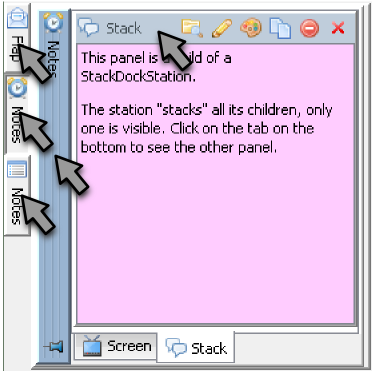
\includegraphics[scale=0.5]{titles}
\caption{Some \src{DockTitles}.}
\label{fig:titles}
\end{figure}

\subsection{Lifecycle}
This chapter will explain the mechanism of creating and managing \src{DockTitle}s. 

A module that wants to show a \src{DockTitle} first has to create a unique identifier. The unique identifier is represented by an instance of \src{DockTitleVersion}. A \src{DockTitleVersion} can be created by the \src{DockTitleManager}. When a module asks for a \src{DockTitleVersion} is has to give a \src{DockTitleFactory} to the manager, this factory becomes the default factory and will be used to create titles (unless someone replaces the default factory).

If the module receives a \src{Dockable} it can call \src{getDockTitle}. This method requires the unique identifier \src{DockTitleVersion} which was created earlier. Most \src{Dockable}s would then access the default factory to create the title, but some \src{Dockable}s might create their customized titles.

Assuming \src{getDockTitle} does not return \src{null}, the module calls the method \src{bind( DockTitle )} of \src{Dockable}, this tells the \src{Dockable} that is has a new title. If the module no longer needs the title it calls \src{unbind( DockTitle )}.

\warningbox{Do not call the method \src{bind} or \src{unbind} of \src{DockTitle}, these methods are called automatically by the \src{DockController}.}

\infobox{\src{Dockable}s provide some information about their titles:
\begin{itemize}
	\item The method \src{listBoundTitles} returns an list of all \src{DockTitle}s which are currently in use for the \src{Dockable}.
	\item A \src{DockableListener} has several methods that will be invoked if titles get added, removed, updated or exchanged.
\end{itemize}}

\subsection{Custom titles}
\subsubsection{Write the title}
It is possible to replace all the titles in the framework. The interface \src{DockTitle} is rather open and the title is responsible to collect the information it wants to show.

Most titles will have a constructor that has a \src{Dockable} as argument. They will add a \src{DockableListener} to their \src{Dockable} once \src{bind} is called and remove the listener once \src{unbind} is called.

Modules that show a title can communicate with the title through the method \src{changed}. This method takes a \src{DockTitleEvent} with further information.

\designbox{A module does not need to know what title it shows. It just delivers the \src{DockTitleEvent} to the title. The module can use a subclass of \src{DockTitleEvent} to transfer more information than \src{DockTitleEvent} alone could carry. This design allows to use any implementation of \src{DockTitle} at any place while some titles still can use additional information from their environment. An example is the \src{EclipseDockTitleEvent} which is used by tabs. This event also tells the titles at which location they are and whether their tab is focused or not.}

There are some classes that can help implementing a custom title:
\begin{itemize}
	\item \src{AbstractDockTitle} provides standard implementations for most of the features a title requires. Subclasses only need to override the method \linebreak \src{paintBackground} to have their custom painting code used.
	\item \src{BasicDockTitle} paints some gradients as background. Clients can change the color of these gradients. This title is also a good reference of how things can be done.
	\item \src{ButtonPanel} is a \src{Component} able to display a set of \src{DockAction}s. \linebreak \src{ButtonPanel} is able to show a popup-menu if there is not enough space for all actions.
\end{itemize}

\classbox{In order to use the popup menu of \src{ButtonPanel} some special code has to be written. First: the argument \src{menu} of the constructor of \src{ButtonPanel} has to be set to \src{true}. Second: the method \src{getPreferredSize} of \src{ButtonPanel} cannot be used, any standard \src{LayoutManager} will fail. Instead the method \src{doLayout} of the \src{Container} which shows the panel can be overriden. In this \src{doLayout} method the container should call \src{getPreferredSizes} to obtain a list of possible sizes of the panel. The $n$'th dimension in this array tells how big the \src{ButtonPanel} would be if it would show $n$ actions. The container should choose the biggest possible $n$ and call \src{setVisibleActions}.}

\subsubsection{Apply the title}
There are three ways to introduce a custom title into the framework.

To override or implement \src{getDockTitle} of \src{Dockable} is the simplest way. The method just creates a new instance of the custom title when called.

The \src{DockTheme} can be used as well. Either override the method \linebreak \src{getTitleFactory} or call \src{setTitleFactory} when using a \src{BasicTheme}. With a few exceptions all the modules use the factory of the theme, hence replacing this factory will have a big effect.

Or use the \src{DockTitleManager} to make some better tuned settings. The \linebreak \src{DockTitleManager} can be accessed by calling \src{getDockTitleManager} of \linebreak \src{DockController}. Search the unique string identifier of the module that uses a title and call \src{getVersion} to access the associated \src{DockTitleVersion}. Then with the help of \src{setFactory} a new factory can be introduced. In code this could look like this:
\begin{lstlisting}
DockController controller = ...

DockTitleManager manager = controller.getDockTitleManager();
DockTitleVersion version =
  manager.getVersion( SplitDockStation.TITLE_ID, null );
version.setFactory( new CustomDockTitleFactory(), Priority.CLIENT );
\end{lstlisting}

\section{Themes}
A \src{DockTheme} relates to \src{DockingFrames} like a \src{LookAndFeel} to \src{Java Swing}. At any given time a \src{DockController} is associated with exactly one theme. The theme defines various graphical elements like icons, painting code and also some behavior code. The current \src{DockTheme} can be changed through the method \src{setTheme}:
\begin{lstlisting}
DockController controller = ...
DockTheme theme = new EclipseTheme();
controller.setTheme( theme );
\end{lstlisting}

\subsection{Existing Themes}
Several \src{DockTheme}s are already included in the framework. A list of theme-factories can be accessed through the method \src{getThemes} of \src{DockUI}. This sub-chapter will list up the existing themes and mention some of their specialities.

Keep in mind that \src{DockTheme}s do not have to follow a specific path for setting up their views. All the current themes are derived from \src{BasicTheme} and thus share a lot of concepts. Future or custom themes however might be implemented in different ways.

\subsubsection{NoStackTheme}
This theme is a wrapper around other themes. It prevents \src{StackDockStation}s from having a \src{DockTitle} and makes sure that the user cannot drag or create a \src{StackDockStation} into another \src{StackDockStation}. The code for creating a \src{NoStackTheme} looks like this:
\begin{lstlisting}
DockTheme original = ...
DockTheme theme = new NoStackTheme( original );
\end{lstlisting}

\subsubsection{BasicTheme}
The \src{BasicTheme} is a simple but working theme. All the other themes of the framework build upon \src{BasicTheme}. This theme shows content whenever possible. It tries to use all features and thus is quite good for debugging, to check whether all features are supported.

\begin{figure}[ht]
\centering
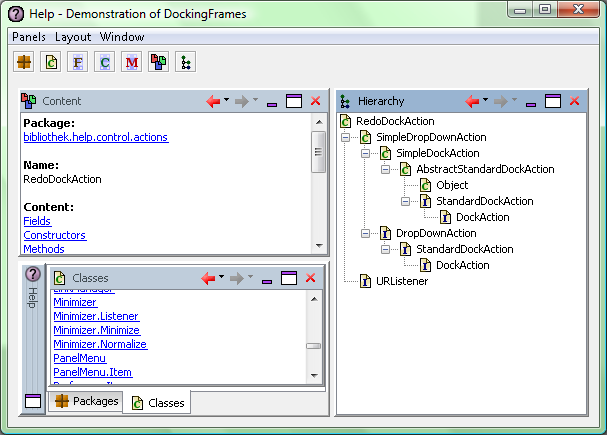
\includegraphics[width=0.5\textwidth]{theme_default}
\caption{BasicTheme}
\label{fig:theme_flat}
\end{figure}

\subsubsection{SmoothTheme}
\src{SmoothTheme} is basically the same as \src{BasicTheme}. The only difference is a replaced default-\src{DockTitleFactory}. As a result new \src{DockTitle}s are used by most elements, these new titles smoothly change their color when the ``active'' state of their \src{Dockable}s changes.

\subsubsection{FlatTheme}
\src{FlatTheme} is a variation of \src{BasicTheme} that tries to minimze the number of borders. Among other things it uses new \src{DockTitle}s and new views for \src{DockAction}s. It is the ideal theme for developers that want to learn how to customize an existing theme.

\begin{figure}[ht]
\centering
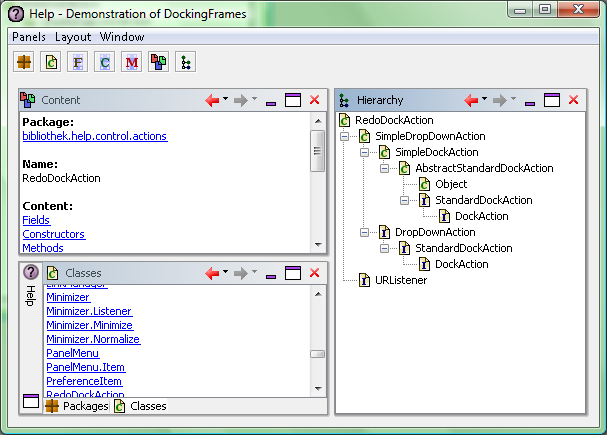
\includegraphics[width=0.5\textwidth]{theme_flat}
\caption{FlatTheme}
\label{fig:theme_basic}
\end{figure}

\subsubsection{BubbleTheme}
A more experimental theme. \src{BubbleTheme} often uses animations and other graphical gimmicks. It has a few performance issues, but it is a good theme to demonstrate the potential of the theme-mechanisms.

\begin{figure}[ht]
\centering
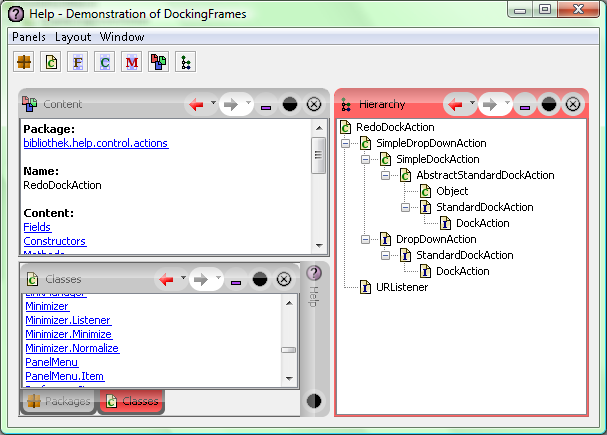
\includegraphics[width=0.5\textwidth]{theme_bubble}
\caption{BubbleTheme}
\label{fig:theme_bubble}
\end{figure}

\subsubsection{EclipseTheme}
\src{EclipseTheme} tries to mimmic the behavior and look of the well known IDE Eclipse. All the \src{Dockable}s are shown on tabbed-components and often \linebreak \src{DockTitle}s are replaced by the tabs. The theme does not use the default theme-mechanisms as often as other themes and it might be a bit tricky to customize the theme. On the other hand it certainly looks good.

\begin{figure}[ht]
\centering
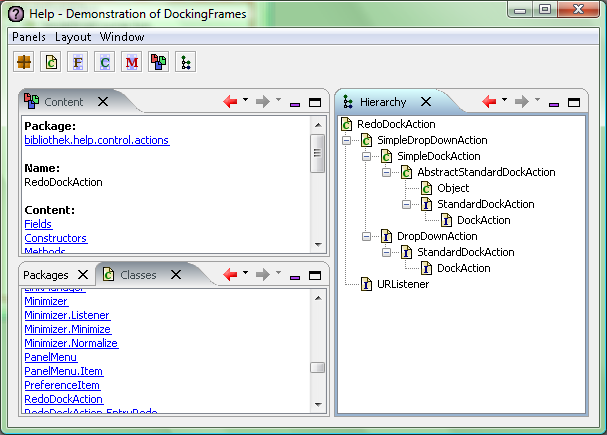
\includegraphics[width=0.5\textwidth]{theme_eclipse}
\caption{EclipseTheme}
\label{fig:theme_eclipse}
\end{figure}

\src{EclipseTheme} offers some keys the map of properties that is stored in \src{DockProperties}. The keys are:
\begin{description}
	\item[PAINT\_ICONS\_WHEN\_DESELECTED] A \src{Boolean} that tells whether \linebreak icons on tabs should be painted if the tab is not selected. In every tabbed-component one tab has to be selected and its associated \src{Dockable} is the only visible element on the component.
	\item[THEME\_CONNECTOR] An \src{EclipseThemeConnector}. The connected tells whether a \src{DockAction} belongs onto a tab, or in a separate list of ``unimportant'' actions. The connector also tells what kind of title to use for a \src{Dockable}.
	\item[TAB\_PAINTER] A \src{TabPainter}. This class is a factory that creates the tab-components and sets up other settings that are related with tabs.
\end{description}

\classbox{The \src{DefaultEclipseThemeConnector} puts every \src{DockAction} which is annotated with \src{EclipseTabDockAction} onto tabs.}

\warningbox{The settings for titles and borders that are given by an \src{EclipseThemeConnector} are not respected if the element is on a \src{StackDockStation}s. A \src{StackDockStation} always uses some tabbed-component.}

\subsection{Customize DockThemes}
More than 50\% of the frameworks source code is only used for painting stuff. No \src{DockTheme} uses particular complex code, just the mass can lead to some loss of direction. This sub-chapter will give only an overview of the basic classes, interfaces and concepts.

\infobox{Many of the mechanisms used by \src{DockTheme}s can be used by clients as well.}

\subsubsection{UI-Properties} \label{sec:uiproperties}
UI-properties is a concept to distribute properties to components. A property could be a \src{Color} and a component some \src{DockTitle} which uses that color to paints it background. The basic idea is to use a map. The keys are \src{String}s, the values are the properties. A \src{DockTheme} or a client can modify or put new key-value pairs into the map and components can read those values which are interesting for them.

Unfortunatelly a simple map is not enough. There needs to be a way to specify values that are used only by a subset of components. Or to remain with the map: the components must become part of the key as well.

The UI-properties provide the necessary features. The mechanism includes these classes, interfaces and generic parameters:
\begin{itemize}
	\item \src{UIProperties}: the base map.
	\item \src{V}: the generic values that have to be distributed, e.g. the class \src{Color}.
	\item \src{UIValue}: A wrapper around \src{V}. Each component creates one \src{UIValue} for each query it will ask the \src{UIProperties}. In example a \src{DockTitle} would have to create and store exactly one \src{UIValue} to represent its background color. \src{UIValue}s also act as observer and the \src{UIProperties} notify an \src{UIValue} if its wrapped \src{V} gets changed.
	\item \src{UIBridge}: An \src{UIBridge} is set between a set of \src{UIValue}s and the \linebreak \src{UIProperties}. \src{V} properties will not be handed directly from \linebreak \src{UIProperties} to \src{UIValue} if there is a bridge between. The bridge can modify the \src{V} property in any way it likes, since the \src{UIBridge} knows the destination of a \src{V} it can also use information derived from the \src{UIValue}.
\end{itemize}

The implementation gets more complex:
\begin{itemize}
	\item For each key several \src{V} properties can be put into the base map. Each value gets assigned another priority (``default'', ``theme'' or ``client'') and only the one with the. highest priority is used.
	\item Each \src{UIValue} is associated with a \src{Path}. The \src{Path} tells what an \src{UIValue} will do with the \src{V} property. The \src{Path} also tells what kind of type the \src{UIValue} has.
	\item \src{UIBridge}s are also associated with a \src{Path}. An \src{UIBridge} is responsible to handle all those \src{UIValue}s that are associated either with the same \src{Path} or a \src{Path} that has the bridges \src{Path} as prefix.
\end{itemize}

\designbox{This scheme allows a flexible handling of resources. On one hand the number of keys is limited and one method call is enough to change a lot things in the user interface (e.g. all background colors of titles). On the other hand clients can implement sophisticated strategies to change some properties without the need to know in detail how the property will be used.

Originally this mechanism was invented to handle \src{Color}s. Then it became evident that the same mechanism could be used for other resources as well. The current implementation requires to implement several classes for each type of resource. While this might be annoying for the first use it ensures type safety. In a system where cause (writing in the map) and effect (reading from the map) can be separated by dozens of classes and an unknown amount of time one does not want to care about types as well.}

\subsubsection{Colors}
In order to understand this chapter \ref{sec:uiproperties} should be read first.

All the colors used in the framework are handled by the \src{ColorManager}. The \src{ColorManager} is an \src{UIProperties} and can be accessed through the \linebreak \src{DockController}. It's use could look like this:
\begin{lstlisting}
DockController controller = ...
ColorManager colors = controller.getColors();
colors.put( Priority.CLIENT, "title.active.left", Color.GREEN );
\end{lstlisting}
In this snippet the value for the key ``title.active.left'' is changed to green. The priority \src{CLIENT} is highest possible priority. It is never overridden by the framework.

Or a more sophisticated use could involve a \src{ColorBridge}:
\begin{lstlisting}
DockController controller = ...
ColorManager colors = controller.getColors();
colors.publish( Priority.CLIENT, TitleColor.KIND_TITLE_COLOR, new ColorBridge(){
	public void add( String id, DockColor uiValue ){
		// ignore
	}
	public void remove( String id, DockColor uiValue ){
		// ignore
	}
	public void set( String id, Color value, DockColor uiValue ){
		TitleColor title = (TitleColor)uiValue;
		if( title.getTitle().getDockable() == <somevalue> )
			title.set( Color.GREEN );
		else
			title.set( value );
	}	
});
\end{lstlisting}
Here a \src{ColorBridge} for the \src{Path} \src{KIND\_TITLE\_COLOR} is installed in line \src{3}. This path is only used by \src{UIValue}s that implement \src{TitleColor}. Hence the unchecked cast from \src{DockColor} to \src{TitleColor} in line \src{11} is safe. The methods \src{add} (line \src{4-6}) and \src{remove} (line \src{7-9}) are called by \src{UIProperties} when a \src{UIValue} gets added or removed to it. These methods can be ignored as long as the bridge does not change the color on its own. Otherwise the \src{DockColor}s could be stored in some list and their method \src{set} could be called whenever the color needs to be exchanged.

This bridge searches for a specific \src{Dockable} called ``somevalue'' (line \src{12}). The bridge returns \src{GREEN} for all colors used by any title of this \src{Dockable}. There is no distinction between the colors for background, foreground or other usages.

\infobox{There is no global list of keys and every \src{DockTheme} uses different keys. All the modules that need colors are annotated with \src{ColorCodes} and expose their own list of keys to the API-documentation. Also the method \src{updateColors} of \src{BasicTheme} or subclasses can help: in this method all the colors that will ever be used by the theme are written into the \src{ColorManager}.}

\classbox{All the standard themes use a \src{ColorScheme} as their initial set of colors. All the standard themes provide a key for the \src{DockProperties} to change that initial scheme. For example the key provided by \src{BasicTheme} is stored as constant \src{BASIC\_COLOR\_SCHEME}. There are several subclasses of \src{ColorScheme} for the different themes.}

By the way: some themes use colors that are read from the current \linebreak \src{LookAndFeel}. Clients can call the method \src{registerColors} of \src{DockUI}. This method takes a \src{LookAndFeelColors} which is responsible in reading the colors from the \src{LookAndFeel}.

\subsubsection{Fonts}
Fonts use the same mechanism as Colors. A \src{FontManager} can be accessed through the methods \src{getFonts} of \src{DockController}. Unlike colors a set of standard keys are defined as constants in \src{DockFont}.

The \src{FontManager} does not distribute \src{Font}-objects but \src{FontModifier}s. A \src{FontModifier} has one method that receives the original \src{Font} and can return any \src{Font} it likes. In example a \src{FontModifier} could inverse the bold-property of a \src{Font}. There are two \src{FontModifiers} ready to use:
\begin{itemize}
	\item \src{ConstantFontModifier} does not modify anything but always return the same \src{Font}
	\item \src{GenericFontModifier} can modify the italic-, bold- and size-property of a font.
\end{itemize}

\classbox{Clients that want to use a \src{FontModifier} might be interested in the classes \src{DLabel} and \src{DPanel} which already modify their font. Also the class \src{FontUpdater} can be used to create new \src{JComponent}s with the capability to modify their font.}

\subsubsection{Icons}
\src{Icon}s can be modified through the \src{IconManager}. The \src{IconManager} is just a map with the capability to inform observers if some of its value changed. The \src{IconManager} can be accessed through the method \src{getIcons} of \linebreak \src{DockController}.

There is no global list of keys in the source code. However the file ``icons.ini'' contains a list of keys and paths of all the default icons.

\subsubsection{Actions}
The views for \src{DockAction}s are changed through the \src{ActionViewConverter}. Please read chapter \ref{sec:actions} for more information.

\subsubsection{Titles}
\src{DockTitle}s are managed by the \src{DockTitleManager}. Please read chapter \ref{sec:titles} for more information.

\subsection{Custom Theme}
With the exception of the classes that are directly related to a \src{DockTheme} no code in the framework depends on a special undocummented behavior of a theme. Clients can reimplement the interface \src{DockTheme} without fear to break things.

A better approach then full reimplementation might be to extend the class \src{BasicTheme}. This class provides some default values which can easily be changed by the appropriate \src{setXZY} method.

\src{DockTheme} has a method \src{install}, this method can be used to exchange some values that are not stored in the \src{DockTheme} itself. For example to exchange icons in the \src{IconManager}.

\warningbox{A theme dives deep into the framework. Implementing a new theme requires a lot of time and a good understanding of the framework. This document might help to understand the basics, but some stuff can only be found out by looking directly at the source code.}

\section{Drag and Drop}
To drag a \src{Dockable} to a new location and drop it there is the most important feature of any docking framework. Surprisingly the implementation of this part is very small.

\subsection{Relocator}
The sourcecode that detects drag gestures, searches for the target station and makes sure that the user has some visual feedback is located in the \linebreak \src{DefaultDockRelocator}. \src{DefaultDockRelocator} itself extends from \linebreak \src{DockRelocator} which just allows to register some listeners and set some useful properties. Clients seldomly need to implement a new \src{DockRelocator}. If they do then they, then they have to implement a new \src{DockControllerFactory}. The code will look like this:

\begin{lstlisting}
public class MyDockControllerFactory extends DefaultDockControllerFactory{
  @Override
  public DockRelocator createRelocator( DockController controller ) {
    return new MyDockReloactor();
  }
}
\end{lstlisting}
This factory has then to be given to the constructor of a \src{DockController}. For the remainder of this chapter it is assumed, that the default relocator is in use.

The \src{DockRelocator} that is in use can be accessed through the method \src{getRelocator} of \src{DockController}.

\subsection{Sources}
The relocator needs to know where and when the user presses and moves the mouse. There is more than one solution for this problem.

\subsubsection{DockElementRepresentative}
A \src{DockElementRepresentative} is a \src{Component} which represents a \src{Dockable}. Anyone can add \src{MouseInputListener}s to a representative and hence be informed about anything the mouse does on top of such a \src{Component}.

\src{DockTitle} and \src{Dockable} are two implementations of \linebreak \src{DockElementRepresentative}. Their registration is handled automatically. If clients implement a new representative then they should call the methods \linebreak \src{addRepresentative} and \src{removeRepresentative} of \src{DockController} to install or uninstall the representative.

\infobox{\src{DockElementRepresentative} was added late to the framework. It carries some legacy code: the method \src{isUsedAsTitle}. This method introduces a distinction between those representations for which all features are activated (e.g. popup menus) and those for which only a selected subset is available. Normally clients implement representatives that are used as title and can return \src{true} here.}

\warningbox{The behavior for representations of \src{Dockable}s that are not registered is unspecified. Clients should not add a \src{DockElementRepresentative} if its \src{Dockable} is unknown to the \src{DockController}.}

\subsubsection{Remote control}
Sometimes it is not possible to implement a \src{DockElementRepresentative}. Remote control of a relocator is an alternative for these cases. Remote control is realized by the classes \src{RemoteRelocator} and \src{DirectRemoteRelocator}.

A \src{RemoteRelocator} can be optained by calling \src{createRemote} of \linebreak \src{DockRelocator}. \src{RemoteRelocator} should be used in combination with a \linebreak \src{MouseListener} and a \src{MouseMotionListener}:
\begin{itemize}
 \item \src{MouseListener.mousePressed} \textrightarrow \src{RemoteRelocator.init}
 \item \src{MouseMotionListener.mouseDragged} \textrightarrow \src{RemoteRelocator.drag}
 \item \src{MouseListener.mouseReleased} \textrightarrow \src{RemoteRelocator.drop}
\end{itemize}
The methods \src{init}, \src{drag} and \src{drop} return a \src{Reaction}. The reaction tells the caller what to do next:
\begin{itemize}
 \item \src{CONTINUE}: the operation continues, the event was ignored.
 \item \src{CONTINUE\_CONSUMED}: the operation continues, the event was consumed. The caller should invoke \src{MouseEvent.consume}.
 \item \src{BREAK}: the operation was canceled, the event was ignored.
 \item \src{BREAK\_CONSUMED}: the operation was canceled, the event was consumed. The caller should invoke \src{MouseEvent.consume}.
\end{itemize}

A \src{DirectRemoteRelocator} can be optained by calling \src{createDirectRemote} of \src{DockRelocator}. A \src{DirectRemoteRelocator} is basically the same as a \src{RemoteRelocator} but always assumes that the user pressed the correct button on the mouse. Its methods do not return a \src{Reaction} because it would always be the same.

\infobox{Clients can use several remote controls at the same time, they will cancel each other out if necessary. A \src{RemoteRelocator} can be used several times.}

\subsection{Destinations}
A relocator needs to find the one \src{DockStation} on which the \src{Dockable} is dropped. 

\subsubsection{Search}
The \src{DefaultDockRelocator} searches the destination anew whenever the mouse is moved. The search includes these steps:
\begin{enumerate}
 \item An ordered list of all potential destinations is built. A \src{DockStation} is a potential destination if it is visible (\src{isStationVisible} of \src{DockStation}), not the dragged \src{Dockable} nor one of its children, and its boundaries contain the location of the mouse (\src{getStationBounds} of \src{DockStation}). The order depends on parent-child relations between the stations, between the \src{Window}s on which the stations are, and on custom conditions that every station can offer (\src{canCompare} and \src{compare} of \src{DockStation}).
 \item Then the method \src{prepareMove} or \src{prepareDrop} of \src{DockStation} is called. These methods check whether the station really is a good destination. They return \src{true} if so, \src{false} if not. The first station that returns \src{true} is the destination.
 \item The method \src{draw} of the new destination is called, the method \src{forget} on the old destination. The new destination will paint some markings to give a visual feedback to the user, the old destination will delete all the information about any drag and drop operation.
\end{enumerate}

\classbox{There is more information about the exact semantics in the API-documentation for \src{DockStation}.}

\subsubsection{Drop}
The moment a user releases the mouse and drops a \src{Dockable} the method \src{move} or \src{drop} of \src{DockStation} is called. These methods can either put the \src{Dockable} somewhere onto the station or merge the \src{Dockable} with an existing child of the station (sometimes referred as ``put'' and ``merge'' action). The results of the first reaction depend on the kind of station. The results of the second reaction are independent of the kind of station.

Merging normally results in creating a new \src{StackDockStation}. The existing child and the dropped \src{Dockable} are put onto that new station. Then the \src{StackDockStation} is put at the place where the existing child was. Creation of ``merged \src{Dockable}s'' is handled by a \src{Combiner}, per default by the \src{BasicCombiner}. Many \src{DockStation}s have a method that allows clients to set their own implementation of a \src{Combiner}. Clients can exchange the \src{Combiner} globally by creating a new \src{DockTheme}, overriding the method \src{getCombiner} and then registering a new instance at the \src{DockController} through \src{setTheme}. Note that all descendants of \src{BasicDockTheme} have a method called \src{setCombiner} that exchanges the \src{Combiner} directly without the need to override \src{getCombiner}.

\warningbox{Exchanging a \src{Combiner} does not affect any existing \src{Dockable} or \src{DockStation}, it will only affect the creation of new elements.}

\subsection{Influences}
There are a number of factors that can influence the search for a new destination. Some of them are customizable.

\subsubsection{Modes}
A \src{DockRelocator} can have "modes". A mode is some kind of behavior that is activated when the user presses a certain combination of keys. Modes are modeled by the class \src{DockRelocatorMode}. It is not specified what effect a mode really has, but normally a mode would add some restrictions where to put a \src{Dockable} during drag and drop. \src{DockRelocatorMode}s can be added or removed to a \src{DockRelocator} by the methods \src{addMode} and \src{removeMode}.

Currently two modes are installed:
\begin{description}
\item[DockRelocatorMode.SCREEN\_ONLY] (press key \textit{shift}) ensures that a \src{Dockable} can only be put on a \src{ScreenDockStation}. That means that a \src{Dockable} can be directly above a \src{DockStation} like a \src{SplitDockStation}, but can't be dropped there.
\item[DockRelocatorMode.NO\_COMBINATION] (press key \textit{alt}) ensures that a \src{Dockable} can't be put over another \src{Dockable}. That means, every operation that would result in a merge is forbidden. Also dropping a \src{Dockable} on already merged \src{Dockable}s will not be allowed.
\end{description}

\classbox{The keys that have to be pressed to activate \src{SCREEN\_ONLY} or \src{NO\_COMBINATION} are the properties \src{SCREEN\_MASK} and \src{NO\_COMBINATION\_MASK}. The can be changed by accessing the \src{DockProperties}.}

\subsubsection{Restrictions}
The set of possible destinations for a \src{Dockable} can be restricted. There are several reasons why a client or the framework itself would do that:
\begin{itemize}
 \item Some \src{Dockable} must always be visible.
 \item Some \src{DockStation}s represent a special area that can only be used by a subset of \src{Dockable}s.
 \item Some \src{Dockable}s can only be presented on a certain kind of \src{DockStation}.
\end{itemize}

This restrictions are implemented through acceptance tests. An acceptance test either checks one ``put'' or one ``merge'' action. Tests can be stored at various locations:
\begin{itemize}
 \item Every \src{Dockable} has two methods called \src{accept}.
 \item Each \src{DockStation} has a method \src{accept}. This method tells whether some \src{Dockable} can become a child of the \src{DockStation}. This method checks ``put'' and ``merge'' actions at the same time.
 \item And then there are \src{DockAcceptance}s. A \src{DockAcceptance} has \src{accept}-methods too. These methods get a \src{DockStation} and some \src{Dockable}s, and then have to decide whether the elements can be put together. Each \src{DockAcceptance} works on a global scale, and thus they are registered at the \src{DockController} through \src{addAcceptance}.
\end{itemize}

\warningbox{Acceptance tests are very powerful. They have to be implemented carefully or the drag and drop mechanism might become crippled.}

************************  was writing here **********************

\section{Preferences}
The preference system was introduced with version 1.0.6 of the core library.

If a setting is meaningful for the ordinary user, and the user would like to be able to change the setting, then this setting should be made accessible through a preference. For example the shortcut to maximize a \src{Dockable} (ctrl+m) is a good candidate for a preference.

So what is a preference? A preference is a representation of some kind of property in a unified way. It is a mediator between the system in which the property is stored, and the graphical user interface and storage mechanisms written for preferences.

Each preference consists of some properties:
\begin{description}
 \item[Value] The thing which the user would like to change.
 \item[ValueInfo] Information about the value, for example the maximum value for an \src{Integer}-value. The exact meaning of this property depends on the \src{TypePath}.
 \item[TypePath] The type tells how to work with the value, how to present it to the user or how to write it as xml. The type is represented by a \src{Path}-object. It is a \src{Path} and not a \src{Class} object because many preference-types may use the same objects as value. For example an unbounded \src{Integer} versus an \src{Integer} which must be in the range 1 to 10.
 \item[Path] A unique path to this preference. Used as an identifier if preferences have to be stored in some kind of map.
\end{description}

\subsection{Organization}
The basic module of the preference system is the \src{PreferenceModel}. 

Most methods of the \src{PreferenceModel} are simple to understand and do not need a discussion. Those which are part of a greater scheme however will receive some attention in this chapter.

In the preference system a \src{PreferenceModel} is just a layer above some kind of storage mechanism for the real properties. It is most often used as a mediator and a buffer between that storage mechanism and the algorithms that want to use the preferences (for example a user interface). The methods \src{read} and \src{write} are used to access the covered storage mechanism. The method \src{read} will read values from the storage mechanism into the model. The method \src{write} will write the values back into that storage mechanism.

\subsection{Models}
There are some implementations of \src{PreferenceModel} already in the core library.

\subsubsection{DefaultPreferenceModel}
This model uses a list of \src{Preference}-objects to represent the preferences. All the properties needed for a preference are stored in such a \src{Preference}-object. The API-documentation reveals that there are many \src{Preference}s representing different aspects of the core library. For example there is a \src{Preference} which represents the keystroke for maximizing a \src{Dockable}.

There are also subclasses of \src{DefaultPreferenceModel}. These subclasses are collections of preferences which belong together, for example the \\\src{EclipseThemePreferenceModel} which contains preferences that are related to the \src{EclipseTheme}.

\subsubsection{MergedPreferenceModel}
This model is a list of other models. It just takes the preferences from these other models and presents them as its own preferences. It offers a quick and simple way to create a combination of two ore more models.

\subsubsection{PreferenceTreeModel}
This model is a \src{PreferenceModel} and a \src{javax.swing.TreeModel}. If seen as \src{PreferenceModel}, then it behaves like a \src{MergedPreferenceModel}. If seen as \src{TreeModel}, then it contains \src{PrefereceTreeModel.Node}-objects. A node can either be just a name, or another \src{PreferenceModel}. This model is intended to be used in a \src{JTree} where the user can select one aspect of the whole set of preferences to show.

The subclass \src{DockingFramesPreferenceModel} is the set of preferences \\which includes all the aspects of the core-library.

\subsection{Lifecycle}
This section describes the best way how to use a \src{PreferenceModel}. Not everything used in this section is explained yet, so you might want to read this section a second time when you finished this whole chapter.

The correct lifecycle of a \src{PreferenceModel} includes normally these steps:
\begin{enumerate}
 \item Create the model. Set up all the preferences that are used by the model.
 \item Call \src{load} on a \src{StoragePreference}.
 \item Call \src{write} on the model to synchronize the model with the underlying system.
 \item (work with the underlying system)
 \item To work with the model: call first \src{read}, then make the changes in the model, then call \src{write}.
 \item (work with the underlying system)
 \item Call \src{read} on the model to synchronize the model with the underlying system.
 \item Store the model using \src{store} of a \src{PreferenceStorage}.
\end{enumerate}

If the \src{PreferenceStorage} used in step \src{2} is empty because its \src{read} or \src{readXML} method failed, then calling \src{read} of \src{PreferenceModel} would at least load some default settings.

Steps \src{4, 5, 6} can be cycled as many times as needed.

An additional step \src{0} and \src{9} would be to read and write the \\\src{PreferenceStorage} when starting up or shuting down the application.

\subsection{User Interface}
If a \src{PreferenceModel} should be displayed, the \src{PreferenceTable} can be used. This table shows a label and an editor for each preference. For \\\src{PreferenceTreeModel}s a \src{PreferenceTreePanel} should be used, it shows a \\\src{PreferenceTable} and a \src{JTree} for the nodes of the \src{PreferenceTreeModel}.

Clients can also use a \src{PreferenceDialog} or a \src{PreferenceTreeDialog} to show a dialog with the well known buttons "ok" and "cancel".

\subsubsection{Editors}
Since there are different types of preferences, different editors are needed. The kind of editor for one preference is determined by the type-path (\src{getTypePath} in a model). Clients can add new editors to a \src{PreferenceTable} through the method \src{setEditorFactory}.

An editor is always of type \src{PreferenceEditor}. Each editor gets a \\\src{PreferenceEditorCallback} with which it can interact with the table. Whenever the user changes the editors value, the editor should call the method \src{set} of \src{PreferenceEditorCallback} to make sure the new value gets stored.

\subsubsection{Operators}
There are some operations which should be available for almost any preference. For example \textit{set a default value} or \textit{delete the current value}. The preference system introduces the \src{PreferenceOperation} to handle this kind of actions.

A \src{PreferenceOperation} is nothing more than a label and an icon. The logic for an operation is either in an editor or in a model.

\begin{description}
 \item[Editor:] Editors with operations must call the method \src{setOperation} of \\\src{PreferenceEditorCallback} for each operation they offer. By calling \src{setOperation} more than once, the editor can change the enabled state of the operation. If the user triggers an operation of the editor, the method \src{doOperation} of \src{PreferenceEditor} is called. It is then the editors responsibility to handle the operation.
 \item[Preference:] Preferences can have operations as well. The method \\\src{getOperations} of \src{PreferenceModel} will be called once to get all the available operations for one preference. The method \src{isEnabled} will be invoked to find out whether an operation is enabled or not. Models can change the enabled state by calling \src{preferenceChanged} of \\\src{PreferenceModelListener}. If the user triggers an operation, \\\src{doOperation} of \src{PreferenceModel} will be invoked.
\end{description}
If an editor and a preference share the same operations, then per definition the operations belong to the editor. All settings from the model will just be ignored.

\subsection{Storage}
The \src{PreferenceStorage} can be used to store \src{PreferenceModel}s in memory or persistent either as byte-stream or as XML.

The normal way to write a model from memory to the disk looks like this:
\begin{lstlisting}
// the stream we want to write into
DataOutputStream out = ...

// the model we want to store
PreferenceModel model = ...

// And now store the model
PreferenceStorage storage = new PreferenceStorage();
storage.store( model );
storage.write( out );
\end{lstlisting}
Note that there are two phases in writing \src{model}. First the model gets \src{store}d (line \src{9}) into \src{storage}. It is possible to store more than just one model in a \src{PreferenceStorage}. Second \src{storage} gets written onto the disk in line \src{10}.

The standard way to read a model are to apply the same steps in reverse:
\begin{lstlisting}
// the source of any new data
DataInputStream in = ...

// the model we want to load
PreferenceModel model = ...

// And now load the model
PreferenceStorage storage = new PreferenceStorage();
storage.read( in );
storage.load( model, false );
\end{lstlisting}
Like writing this operation has two phases. In line \src{9} \src{storage} gets filled with information, in line \src{10} the information gets transfered to \src{model}. The argument \src{false} is a hint what to do with missing preferences. In this case missing preferences are just ignored. A value of \src{true} would force them to become \src{null}.

There are some preferences which do not need to be stored by the \\\src{PreferenceStorage} because they are already stored by the underlying systen. These preferences are called \textit{natural}, while the others are called \textit{artificial}. The method \src{isNatural} of \src{PreferenceModel} can be used to distinguish them.

\section{Properties}

\end{document} 